\ylDisplay{Nurgapeegel} % Ülesande nimi
{Andreas Valdmann} % Autor
{lõppvoor} % Voor
{2016} % Aasta
{G 8} % Ülesande nr.
{8} % Raskustase
{
% Teema: Geomeetriline-optika
\ifStatement
\begin{wrapfigure}{r}{0.35\textwidth}
	\vspace{-25pt}
	\begin{center}
		
\includegraphics[width=0.35\textwidth]{2016-v3g-08-wink.png}
	\end{center}
	\vspace{-20pt}
\end{wrapfigure}

Jukul oli katsetamiseks kolm ruudukujulist tasapeeglit. Ühte peeglisse vaadates ja paremat silma kinni pigistades nägi ta endast joonisel kujutatud peegelpilti. Järgmisena paigutas Juku kolm peeglit sedasi, et need moodustasid kuubi kolm tahku, millel on üks ühine tipp. Sealjuures jäid peegelpinnad kuubi sisemisele poolele. Joonistage peegelpilt, mida paremat silma kinni pigistav Juku endast otse nurgapeegli nurka vaadates nägi ja põhjendage tulemust konstrueerimise teel.
\fi


\ifHint
Juku näo kujutise leidmiseks tasub kõigepealt vaadelda, kuidas Juku silmad peeglites kujutisi tekitavad. Kuna peeglid on üksteise suhtes täisnurga all, on selge, et otse nurgapeegli nurka vaadates on näha kolmandat järku kujutis.
\fi


\ifSolution
Vaatame kõigepealt kujutise tekkimist tasapeeglis. Joonisel 1 on olukord pealtvaates. A on Juku lahtine silm ja A$'$ selle kujutis. Kinnine silm  ja selle kujutis on vastavalt B ja B$'$. Näeme, et parema silma kinnipigistamisel paistab ka peeglis kinnisena vaatleja suhtes parempoolne silm.
\begin{figure*}[h]
	\centerline{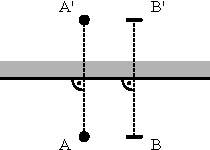
\includegraphics[scale=1.2]{2016-v3g-08-nurgapeegel_j1}}
	\caption{Kujutis tasapeeglis}
\end{figure*}

Olgu kolmest peeglist üks horisontaalne ja kaks ülejäänut vertikaalsed, kusjuures Juku vaatab otse vertikaalsete peeglite kokkupuutejoone poole. Joonisel 2 on see olukord pealtvaates. Vaatame vertikaalsete peeglite mõju. Esmalt konstrueerime silma A kujutise A$'$ vasakpoolses peeglis. Seejärel konstrueerime kujutise A$'$ kujutise A$''$ parempoolses peeglis. Toimime samamoodi kujutise B$''$ konstrueerimisel ja paneme tähele, et seekord on peegelpildil vasak ja parem pool vahetatud ning kinnisena paistab peeglites vasakpoolne silm.
\begin{figure*}[h]
	\centerline{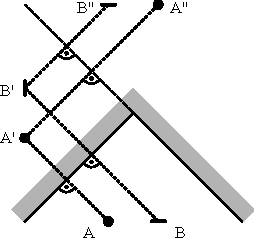
\includegraphics[scale=1.2]{2016-v3g-08-nurgapeegel_j2}}
	\caption{Kujutis kahes peeglis}
\end{figure*}

Võtame nüüd arvesse horisontaalse peegli mõju. Joonisel 3 on otsevaates teist järku kujutis A$''$ ning selle kujutis A$'''$ horisontaalses peeglis. Näeme, et horisontaalne peegel pöörab pildi \enquote{pea peale}. Seega näeb Juku nurgapeeglis ennast sellisena, nagu on joonisel 3 kujutis A$'''$.
\begin{figure*}[h]
	\centerline{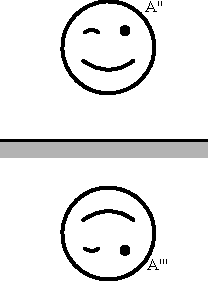
\includegraphics[scale=1.1]{2016-v3g-08-nurgapeegel_j3}}
	\caption{Peegeldumine horisontaalselt peeglilt}
\end{figure*}
\fi


\ifEngStatement
% Problem name: Corner mirror
\begin{wrapfigure}{r}{0.3\textwidth}
	\vspace{-25pt}
	\begin{center}
		
\includegraphics[width=0.3\textwidth]{2016-v3g-08-wink}
	\end{center}
	\vspace{-20pt}
\end{wrapfigure}
Juku had three square-shaped plane mirrors for experimenting. Looking at one mirror and squeezing his right eye he saw the reflection depicted in the figure. Next, Juku positioned the three mirrors so that they formed the three faces of a cube that had a common tip. The reflecting faces of the mirrors stayed on the inner side of the cube. Sketch the reflection of himself that Juku saw while closing his right eye and looking exactly at the common vertex of the mirrors. Explain by construction.
\fi


\ifEngHint
To find the image of Juku’s face you should first observe how Juku’s eyes create images in the mirrors. Because the mirrors are at right angle with respect to each other it is clear that looking straight at the corner of the corner mirror a third stage image would be seen.
\fi


\ifEngSolution
Let us first study the formation of an image in a flat mirror. The situation is pictured in the figure 1 from top view. A is Juku’s open eye and A$'$ its image. A closed eye and its image are respectively B and B$'$. We see that if one closes the right eye then with respect to the observer the right eye in the mirror seems to be closed as well. 
\begin{figure*}[h]
	\centerline{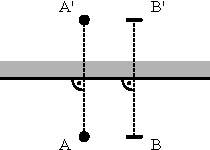
\includegraphics[scale=1.2]{2016-v3g-08-nurgapeegel_j1}}
	\caption{Image in a plane mirror}
\end{figure*}
Let one of the mirror from the three be horizontal and the two rest vertical, moreover Juku looks directly to the line between the vertical mirrors. In the figure 2 this situation is pictured from top view. Let us observe the effect of the vertical mirrors. First, we construct the image A$'$ of the eye A in the left mirror. Next we construct the image A$''$ of the image A$'$ in the right mirror. We do the same when constructing the image B$''$ and notice that this time the right and left side of the reflection are switched and the eye that seems to be closed is the left one.\\
Let us now take into consideration the impact of the horizontal mirror. In the figure 3 the second order image A$''$ and its image A$'''$ are in front view. We see that the horizontal mirror reverses the picture. Therefore Juku sees himself from the corner mirror as the image A$'''$ from the figure 3. 
\begin{figure*}[h]
	\centerline{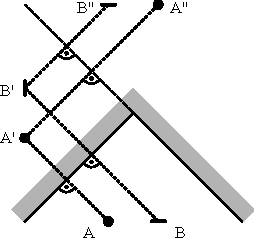
\includegraphics[scale=1.2]{2016-v3g-08-nurgapeegel_j2}}
	\caption{Image in two mirrors}
\end{figure*}
\begin{figure*}[h]
	\centerline{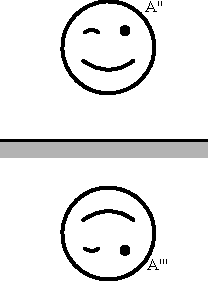
\includegraphics[scale=1.1]{2016-v3g-08-nurgapeegel_j3}}
	\caption{Reflection from horizontal mirror}
\end{figure*}
\fi
}